\section{Aufbau}
\label{sec:Aufbau}
Eine Wärmepumpe kann schematisch wie folgt dargestellt werden:
\begin{figure}
  \centering
  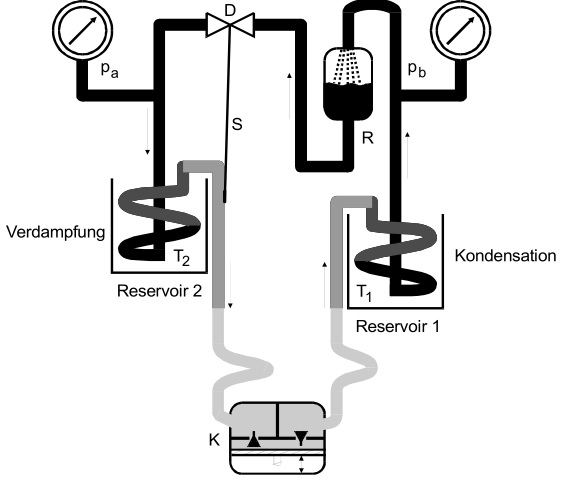
\includegraphics{data/Abb1.jpg}
  \caption{Prinzipieller Aufbau einer Wärmepumpe. \cite{AnleitungV206}}
  \label{fig:Abb1}
\end{figure}
Für die Wärmepumpe wird ein reales Gas benutzt, welches während des Verdampfens Wärme aufnimmt und bei der Kondensation abgibt.
Dies ist die Phasenumwandlungsenergie einer transportablen Energie des Gases.
Für eine ideal arbeitende Pumpe sollte das Gas eine möglichst hohe Kondensationswärme besitzen.
Der Kompressor K sorgt für eine adiabatische Kompression und einen Kreislauf.
Das Druckventil D lässt druckreguliert das Gas durchströmen.
Dort liegt ein Druckunterschied zwischen den beiden Reservoiren vor.
Das Transportmedium mit dem Druck $p_b$ und der Temperatur $T_1$ ist flüssig,
während es auf der anderen Seite bei $p_a$ mit der Temperatur $T_2$ gasförmig ist.
Wenn sich das Drosselventil D öffnet, entzieht es dem Wasser in Reservoir 2 die Verdampfungswärme L.
Somit ist das Reservoir 2, das kältere, wärmespendende Gefäß ist.
Das Gas strömt durch den Kompressor K, wird komprimiert und erwärmt sich somit.
Dadurch steigt der Druck im Reservoir $p_a$ , bis sich das Gas verflüssigt und somit Wärme an das Gefäß abgibt.
Mittels weiterer Apparaturen, wie dem Reiniger R werden Blasen durch die Entfernung von Gasresten entfernt,
oder der Steuervorrichtung S, welche das Drossenventil D reguliert.
Dadurch wird sichergestellt, dass nur Gase in den Kompressor gelangen.
